
\question
{\center \bf Sliding Image Puzzle\\}
You have been assigned to develop a program that will aid a {\bf sliding
image puzzle} manufacturer in partitioning images for their puzzles.

\begin{figure}[H]
\centering
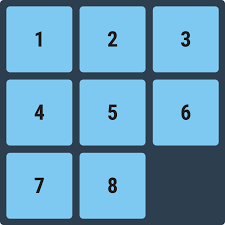
\includegraphics[scale=.5]{sliding_puzzle.png}
\caption{Sliding Puzzle}
\end{figure}

The program should be designed to accomplish the following tasks:

\begin{itemize}
\item \textbf{Task 1} Read \verb|images.txt|, which contains the links to the images.
 \begin{figure}[H]
  \centering
  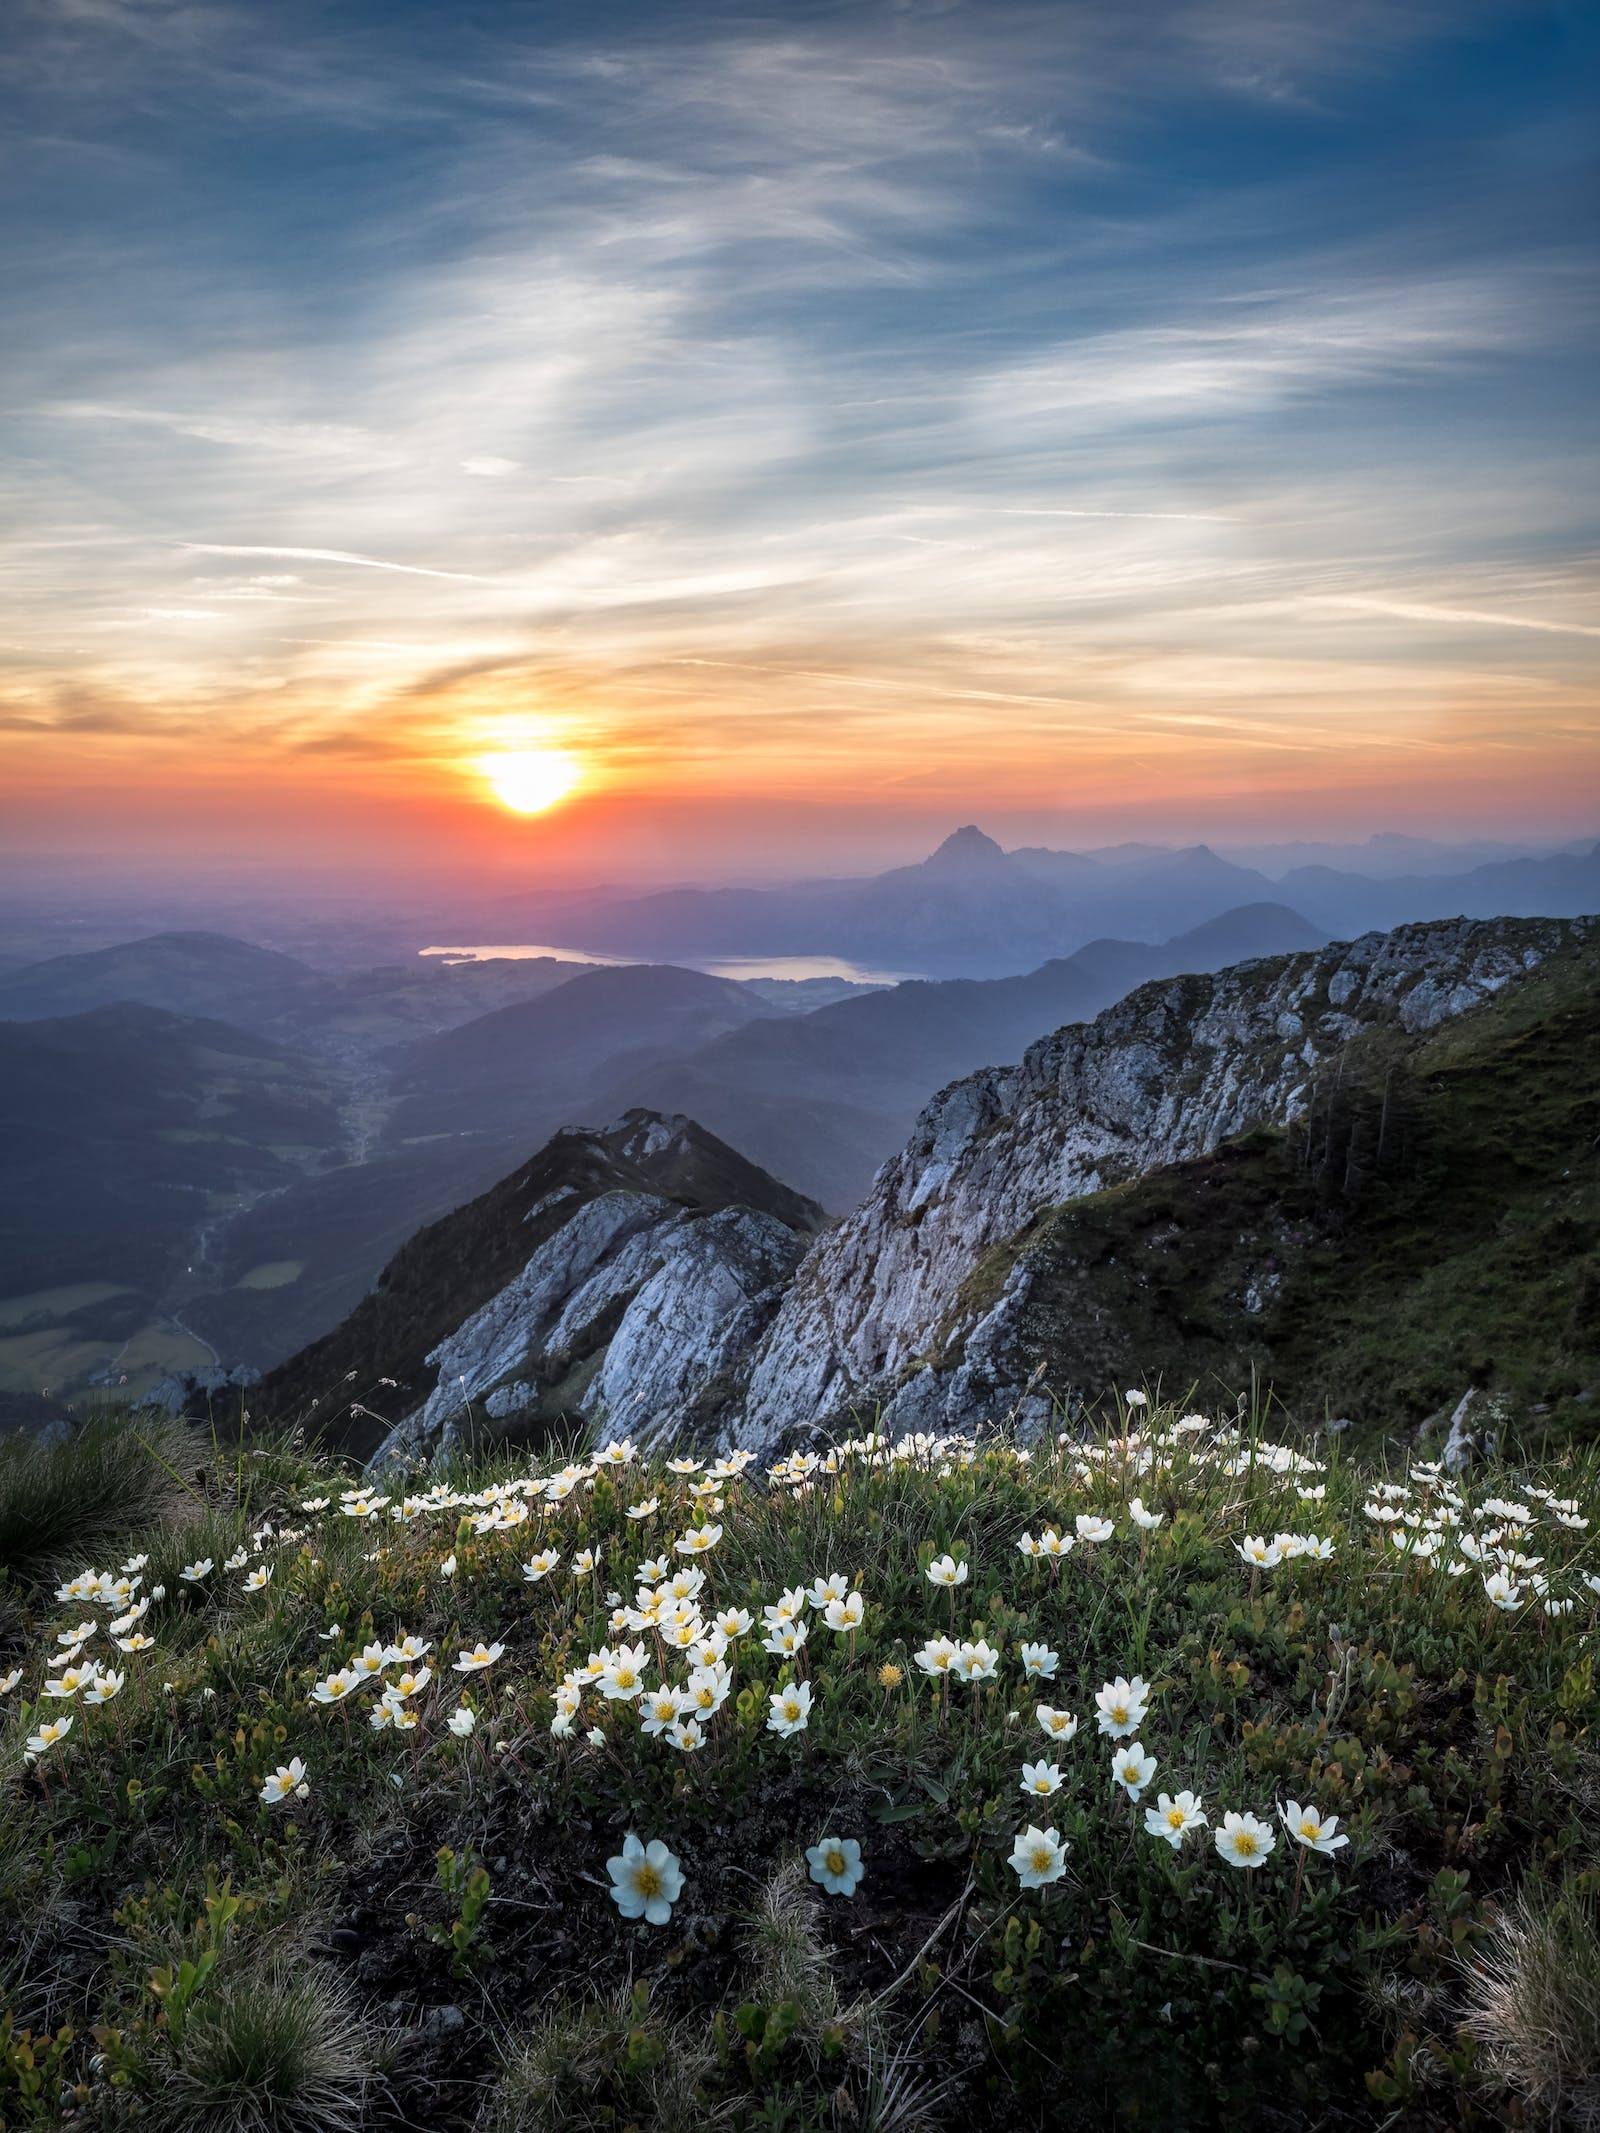
\includegraphics[scale=.088]{nature.jpeg}
  \end{figure}
  \href{https://ydjemmada.github.io/projects/images.txt}{Click here to get images.txt}
\item \textbf{Task 2} For images that are not square-shaped, crop them to obtain the maximum-sized square image possible located in the middle of the original image.
\begin{figure}[H]
\centering
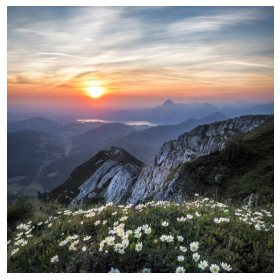
\includegraphics[scale=.5]{image_croped.png}
\end{figure}

\item \textbf{Task 3} Partition each image into eight equal parts, as
  illustrated in the the follwing figure.

\begin{figure}[H]
\centering
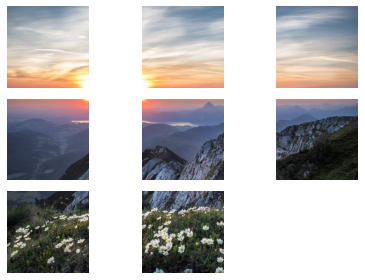
\includegraphics[scale=.5]{image_order.png}
\end{figure}


\item \textbf{Task 4} Generate a permuted grid of the eight small parts of the cropped image.

\begin{figure}[H]
\centering
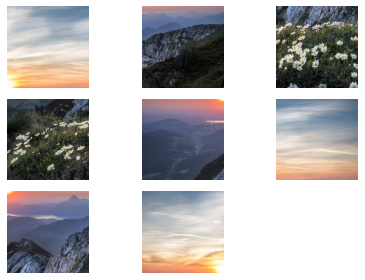
\includegraphics[scale=.5]{image_slides.png}
\end{figure}

\item \textbf{Task 5} Store each cropped image and its corresponding eight small parts in a directory named \verb|puzzle_i|, where \verb|i| represents the image's order in the file.
\end{itemize}

Your program should be programmed to perform these tasks effectively and
efficiently. It should be thoroughly documented, and clear instructions
should be provided to your users.
\newpage